\documentclass[12pt,-letter paper]{article}
\usepackage{graphicx}
\usepackage{enumitem}
\usepackage{tfrupee}
\usepackage{amsmath}
\usepackage{amssymb}
\usepackage{mwe} % for blindtext and example-image-a in example
\usepackage{wrapfig}
\graphicspath{sdcard/pics/math.png}

\title{Matrix assignment}
\date{\today}

\begin{document}

\maketitle{Questions}
\begin{enumerate}
	\item The pair of linear equations 2x=5y+6 and 15y=6x-18 represents two lines which are : 
\begin{enumerate}
    \item intersecting
    \item parallel
    \item coincident
    \item either intersecting or parallel
\end{enumerate}
\item Two schools 'P'and 'Q' decided to award prizes to their students for two games of Hockey \rupee \textit{x} per students and cricket \rupee \textit{y} per student. School 'P'
decided to award a total of \rupee 9,500 for the two games to 5 and 4 students respectively; while school 'Q' decided to award \rupee 7,370 for the two games to 4 and 3 students respectively.
\begin{figure}
    \centering
    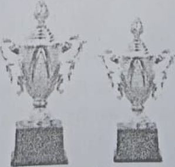
\includegraphics{math.png}

\caption{}
\end{figure}
\\Based on the given information, answer the following questions :
\begin{enumerate}[label=(\roman*)]
    \item Represent the following information algebraically(in terms of \textit{x} and \textit{y}).
    \item\begin{enumerate}[label=(\alph*)]
\item what is the prize amount for hockey ?
    \begin{center}{\textbf{OR}}
\end{center}
\item Prize amount on which game is more and by how much ?
    
    \end{enumerate}
    \item what will be the total prize amount if there are 2 students each from two games ?
\end{enumerate}
\item If the pair of equations 3x- y + 8 = 0 and 6x - ry +16 =0 represents coincident lines,then the values of '\textit{r}' is :
\begin{enumerate}[label=(\alph*)]
    \item $-\frac{1}{2}$
    \item $\frac{1}{2}$
    \item 2
    \item -2
\end{enumerate}
\item The pair of equations x=a and y=b graphically represents lines which are :
\begin{enumerate}[label=(\alph*)]
    \item parallel
    \item intersecting at (b,a)
    \item coincident
    \item intersecting at (a,b)
    
\end{enumerate}
\item
\begin{enumerate}[label=(\alph*)]
\item If the system of linear equations \newline 2x + 3y = 7 and  2ax +(a + b)y =28 \newline have infinite number of solutions, then find the values of 'a' and 'b'.
\begin{center}{\textbf{OR}}
\end{center}
\item  If 217x + 131y = 913 and \newline
131x + 217y = 827,\newline then solve the equations for the values of x and y.
\end{enumerate}
\item Half of the difference between two numbers is 2. The sum of the greater number and twice the smaller number is 3.Find the numbers.\newpage
\item If (a ,b),(c, d) and (e, f) are the vertices of $\Delta$ABC and $\Delta$ denotes the area of $\Delta$ABC, then 
\begin{math}
   \begin{vmatrix}
a & c & e\\
b & d& f\\
1&1&1
\end{vmatrix}^2 
\end{math}
 is equal to
\begin{enumerate}[label=(\alph*)]
    \item 2$\Delta ^2$
    \item 4$\Delta ^2$ 
    \item 2$\Delta$
    \item 2$\Delta$
\end{enumerate}
    \item If 
\begin{math}
\begin{bmatrix}
2 & 0 \\
5 & 4 
\end{bmatrix} = P + Q
\end{math}
is a symmetric and Q is a skew symmetric matrix, then Q is equal to
\begin{enumerate}[label=(\alph*)]
    \item \begin{math}
\begin{bmatrix}
2  & \frac{5}{2} \\
 \frac{5}{2} & 4 
\end{bmatrix} 
\end{math}
    \item \begin{math}
\begin{bmatrix}
0 & -\frac{5}{2} \\
\frac{5}{2} & 0 
\end{bmatrix} 
\end{math}
    \item \begin{math}
\begin{bmatrix}
0 & \frac{5}{2} \\
-\frac{5}{2} & 0 
\end{bmatrix}
\end{math}
    \item \begin{math}
\begin{bmatrix}
2 & -\frac{5}{2} \\
\frac{5}{2} & 4 
\end{bmatrix}
\end{math} 
\end{enumerate}
\item If \begin{math}
\begin{bmatrix}
1 & 2 & 1 \\
2 & 3 & 1 \\
3 & a & 1
\end{bmatrix}
\end{math} is non-singular matrix and  $a \in A $, then the set A is 
\begin{enumerate}[label=(\alph*)]
    \item $\mathbb{R}$
    \item \{0\}
    \item \{4\}
    \item $\mathbb{R}$-\{4\}
\end{enumerate}
\newpage
\item If\begin{math}
     \begin{vmatrix}
    A
\end{vmatrix} = \begin{vmatrix}
    kA
\end{vmatrix}
\end{math}, where A is a square matrix of order 2,then sum of all possible values of k is
\begin{enumerate}[label=(\alph*)]
    \item 1
    \item -1
    \item 2
    \item 0
\end{enumerate}
\item
\begin{enumerate}[label=(\alph*)]
    \item 
If A=\begin{math}
\begin{bmatrix}
    -3 & -2 & -4\\
    2 & 1 & 2\\
    2 & 1 & 3
\end{bmatrix}
\end{math}
and B =\begin{math}
\begin{bmatrix}
    1 & 2 & 0\\
    -2 & -1 & -2\\
    0 & -1 & 1
\end{bmatrix}
\end{math},then find AB and use it to solve the following system of equations :
\\x - 2y = 3
\\2x - y - z = 2
\\-2y + z = 3
\begin{center}{\textbf{OR}}
\end{center}
\item If f\((\alpha)\)=\begin{math}
\begin{bmatrix}
    cos\alpha & -sin\alpha & 0\\
    sin\alpha & cos\alpha & 0\\
    0 & 0 & 1
\end{bmatrix}
\end{math} ,then prove that f\((\alpha)\).f\((-\beta)\) = f\((\alpha - \beta)\).
\end{enumerate}
 \end{enumerate}
\end{document}
